% vim: set spelllang=fr:
\documentclass{main}

\title{\textbf{Séance 3}\\Graphes (partie 2)}
\institute{Université de Montpellier}
\author{Mattéo Delabre}
\date{14 février 2021}

\begin{document}

\begin{frame}{Programme d’entraînement}
    \begin{itemize}
        \item 31 janvier --- Introduction et stratégies de recherche
        \item 7 février --- Graphes (partie 1)
        \item \textbf{14 février --- Graphes (partie 2)}
        \item Semaine du 22 au 28 février --- Chaînes de caractères
        \item Semaine du 22 au 28 février --- Géométrie algorithmique
        \item Semaine du 22 au 28 février --- Concours blanc
        \item 28 février --- Concours blanc
        \item 6 et 7 mars --- SWERC
    \end{itemize}
\end{frame}

\maketitle

\begin{frame}{Suite du programme}
    Précédemment dans le monde des graphes :\begin{itemize}
        \item Couplages maximums
        \item Problème d’affectation (algorithme hongrois)
        \item Tri topologique
        \item Plus long chemin dans un arbre (diamètre)
        \item Cycles et chemins eulériens
        \vspace{8pt}
        \hrule
        \vspace{8pt}
        \item Plus courts chemins
        \item Arbre couvrant de poids minimum
        \item Composantes (fortement) connexes
        \item Mariages stables
    \end{itemize}
    
    \textbf{Dans cette présentation : Maximisation de flots.}
\end{frame}

\section{Introduction}
\maketoc

\pgfkeys{
    /tikz/on layer/.code={
        \pgfonlayer{#1}\begingroup
        \aftergroup\endpgfonlayer
        \aftergroup\endgroup
    },
}

\tikzset{
    pipe/.style={
        draw, white,
        rounded corners,
        line width=sqrt(#1)*4pt-2pt,
        preaction={
            on layer=back,
            draw, curseblue,
            rounded corners,
            line width=sqrt(#1)*4pt,
        }
    },
    water/.style={
        draw, blue!20,
        rounded corners,
        line width=sqrt(#1)*4pt-2pt,
    },
    weight/.style={
        curseblue,
        font=\footnotesize,
    },
    graph node/.style={
        draw, circle,
    }
}

\newcommand\pipenode[2]{
    \fill[curseblue, on layer=back] (#1) circle (#2*1pt);
    \fill[white, onslide=<2>{blue!20}] (#1) circle (#2*1pt-1pt);
}

\begin{frame}{Exemple introductif}
Quel est le plus grand débit d’eau possible en sortie du système ?
\vspace{1em}

\centering
\begin{tikzpicture}[x=2cm]
    \coordinate (s) at (0, 0);
    \coordinate (1) at (1, 1);
    \coordinate (2) at (2, 1);
    \coordinate (3) at (1, -1);
    \coordinate (4) at (2, -1);
    \coordinate (t) at (3, 0);
    
    \draw[pipe=7] ($(s)-(.2,0)$) -- (s);
    \only<2>{\draw[water=7] ($(s)-(.2,0)$) -- (s);}
    
    \draw[pipe=5] (s) |- node[
        pos=.75, weight,
        yshift=12pt,
    ] {\only<2>{3/}5 $\ell$/min} (1);
    \only<2>{\draw[water=3] (s) |- (1);}
    
    \draw[pipe=4] (s) |- node[
        pos=.75, weight,
        yshift=-12pt,
    ] {\only<2>{4/}4 $\ell$/min} (3);
    \only<2>{\draw[water=4] (s) |- (3);}
    
    \draw[pipe=3] (1) -- node[
        midway, weight,
        xshift=-18pt,
        align=right,
    ] {\only<2>{3/}3\\$\ell$/min} (3);
    \only<2>{\draw[water=3] (1) -- (3);}
    
    \draw[pipe=6] (1) -- node[
        midway, weight,
        yshift=12pt,
    ] {\only<2>{6/}6 $\ell$/min} (2);
    \only<2>{\draw[water=6] (1) -- (2);}
    
    \draw[pipe=1] (3) -- node[
        midway, weight,
        yshift=-12pt,
    ] {\only<2>{1/}1 $\ell$/min} (4);
    \only<2>{\draw[water=1] (3) -- (4);}
    
    \draw[pipe=8] (2) -- node[
        midway, weight,
        xshift=-22pt,
        align=right,
    ] {\only<2>{1/}8\\$\ell$/min} (4);
    \only<2>{\draw[water=1] (2) -- (4);}
    
    \draw[pipe=5] (2) -| node[
        pos=.25, weight,
        yshift=12pt,
    ] {\only<2>{5/}5 $\ell$/min} (t);
    \only<2>{\draw[water=5] (2) -| (t);}
    
    \draw[pipe=2] (4) -| node[
        pos=.25, weight,
        yshift=-12pt,
    ] {\only<2>{2/}2 $\ell$/min} (t);
    \only<2>{\draw[water=2] (4) -| (t);}
    
    \draw[pipe=7] ($(t)+(.2,0)$) -- (t);
    \only<2>{\draw[water=7] ($(t)+(.2,0)$) -- (t);}
    
    \node[left=of s, align=right]
        {source\only<2>{\\7 $\ell$/min}};
    \node[right=of t, align=left]
        {puits\only<2>{\\7 $\ell$/min}};
    
    \pipenode{s}{8}
    \pipenode{1}{8}
    \pipenode{2}{8}
    \pipenode{3}{8}
    \pipenode{4}{8}
    \pipenode{t}{8}
\end{tikzpicture}%
\end{frame}

\section{Réseaux et problème de maximisation de flot}
\maketoc

\begin{frame}{Généralisons un peu}
Quel est la valeur maximum d’un flot dans ce graphe?

\centering
\begin{tikzpicture}[x=2cm]
    \node[graph node] (s) at (0, 0) {$s$};
    \node[graph node] (1) at (1, 1) {$1$};
    \node[graph node] (2) at (2, 1) {$2$};
    \node[graph node] (3) at (1, -1) {$3$};
    \node[graph node] (4) at (2, -1) {$4$};
    \node[graph node] (t) at (3, 0) {$t$};
    
    \draw (s) -- node[
        midway, weight,
        yshift=12pt,
    ] {3/5} (1);
    \draw (s) -- node[
        midway, weight,
        yshift=-12pt,
    ] {4/4} (3);
    \draw (1) -- node[
        midway, weight,
        xshift=-12pt,
    ] {3/3} (3);
    \draw (1) -- node[
        midway, weight,
        yshift=12pt,
    ] {6/6} (2);
    \draw (3) -- node[
        midway, weight,
        yshift=-12pt,
    ] {1/1} (4);
    \draw (2) -- node[
        midway, weight,
        xshift=-12pt,
    ] {1/8} (4);
    \draw (2) -- node[
        midway, weight,
        yshift=12pt,
    ] {5/5} (t);
    \draw (4) -- node[
        midway, weight,
        yshift=-12pt,
    ] {2/2} (t);
\end{tikzpicture}

\begin{itemize}
    \item Données dans un réseau informatique
    \item Trains dans un réseau ferroviaire
    \item Marchandises dans une chaîne logistique
\end{itemize}
\end{frame}

\begin{frame}{Utilité de ce problème}
    \begin{itemize}
        \item Algorithmes de résolution efficaces
        \begin{itemize}
            \item \textbf{Edmonds-Karp : $O(|V|\times|E|^2)$}
            \item Dinic : $O(|V|^2\times|E|)$
        \end{itemize}
        \item Grand pouvoir de modélisation
        \begin{itemize}
            \item Nombre maximum de chemins disjoints
            \item Résilience d’un réseau
            \item Couplage maximal dans un biparti
            \item Élimination d’équipes au baseball
        \end{itemize}
    \end{itemize}
\end{frame}

\section{Algorithme pour trouver un flot maximum}
\maketoc

\tikzset{
    highlight/.style={
        ultra thick, red!90!curseblue,
    },
    highlight green/.style={
        ultra thick, green!60!curseblue,
    }
}

\begin{frame}{Premier algorithme glouton}
Rechercher des plus courts chemins augmentants, tant que c’est possible.
S’il n’y en a plus, c’est qu’on a trouvé un flot maximum.

\vspace{1em}
\centering
\begin{tikzpicture}[x=2cm, >=Latex]
    \node[graph node] (s) at (0, 0) {$s$};
    \node[graph node] (1) at (1, 1) {$1$};
    \node[graph node] (2) at (2, 1) {$2$};
    \node[graph node] (3) at (1, -1) {$3$};
    \node[graph node] (4) at (2, -1) {$4$};
    \node[graph node] (t) at (3, 0) {$t$};
    
    \draw[
        ->,
        onslide=<2>{highlight},
    ] (s) -- node[
        midway, weight,
        yshift=12pt,
        onslide=<2>{highlight},
    ] {\only<1>{0}\only<2->{5}/5} (1);
    
    \draw[
        ->,
        onslide=<3-4>{highlight},
    ] (s) -- node[
        midway, weight,
        yshift=-12pt,
        onslide=<3-4>{highlight},
    ] {\only<1-2>{0}\only<3>{1}\only<4>{2}/4} (3);
    
    \draw[
        ->,
        onslide=<4>{highlight},
    ] (3) -- node[
        midway, weight,
        xshift=-12pt,
        onslide=<4>{highlight},
    ] {\only<1-3>{0}\only<4>{1}/3} (1);
    
    \draw[
        ->,
        onslide=<2>{highlight},
        onslide=<4>{highlight},
    ] (1) -- node[
        midway, weight,
        yshift=12pt,
        onslide=<2>{highlight},
        onslide=<4>{highlight},
    ] {\only<1>{0}\only<2-3>{5}\only<4>{6}/6} (2);
    
    \draw[
        ->,
        onslide=<3>{highlight},
    ] (3) -- node[
        midway, weight,
        yshift=-12pt,
        onslide=<3>{highlight},
    ] {\only<1-2>{0}\only<3->{1}/1} (4);
    
    \draw[
        ->,
        onslide=<4>{highlight},
    ] (2) -- node[
        midway, weight,
        xshift=-12pt,
        onslide=<4>{highlight},
    ] {\only<1-3>{0}\only<4>{1}/8} (4);
    
    \draw[
        ->,
        onslide=<2>{highlight},
    ] (2) -- node[
        midway, weight,
        yshift=12pt,
        onslide=<2>{highlight},
    ] {\only<1>{0}\only<2->{5}/5} (t);
    
    \draw[
        ->,
        onslide=<3-4>{highlight},
    ] (4) -- node[
        midway, weight,
        yshift=-12pt,
        onslide=<3-4>{highlight},
    ] {\only<1-2>{0}\only<3>{1}\only<4>{2}/2} (t);
\end{tikzpicture}
\end{frame}

\begin{frame}{Contre-exemple}
\centering
\begin{tikzpicture}[x=2cm, >=Latex]
    \node[graph node] (s) at (0, 0) {$s$};
    \node[graph node] (1) at (1, -1) {$1$};
    \node[graph node] (2) at (2, -1) {$2$};
    \node[graph node] (3) at (2, 1) {$3$};
    \node[graph node] (4) at (3, 1) {$4$};
    \node[graph node] (t) at (4, 0) {$t$};
    
    \draw[
        ->,
        onslide=<3>{highlight},
    ] (s) -- node[
        midway, weight,
        yshift=-12pt,
        onslide=<3>{highlight},
    ] {\only<1-2>{0}\only<3->{9}/10} (1);
    
    \draw[
        ->,
        onslide=<2>{highlight},
        onslide=<4>{highlight},
    ] (s) to[bend left=10] node[
        midway, weight,
        yshift=12pt,
        onslide=<2>{highlight},
        onslide=<4>{highlight},
    ] {\only<1>{0}\only<2-3>{1}\only<4->{10}/10} (3);
    
    \draw[
        ->,
        onslide=<2-3>{highlight},
    ] (2) to[bend right=10] node[
        midway, weight,
        yshift=-12pt,
        onslide=<2-3>{highlight},
    ] {\only<1>{0}\only<2>{1}\only<3->{10}/10} (t);
    
    \draw[
        ->,
        onslide=<4>{highlight},
    ] (4) -- node[
        midway, weight,
        yshift=12pt,
        onslide=<4>{highlight},
    ] {\only<1-3>{0}\only<4->{9}/10} (t);
    
    \draw[
        ->,
        onslide=<3>{highlight},
    ] (1) -- node[
        midway, weight,
        yshift=-12pt,
        onslide=<3>{highlight},
    ] {\only<1-2>{0}\only<3->{9}/10} (2);
    
    \draw[
        ->,
        onslide=<2>{highlight},
    ] (3) -- node[
        midway, weight,
        xshift=-12pt,
        onslide=<2>{highlight},
    ] {\only<1>{0}\only<2->{1}/1} (2);
    
    \draw[
        ->,
        onslide=<4>{highlight},
    ] (3) -- node[
        midway, weight,
        yshift=12pt,
        onslide=<4>{highlight},
    ] {\only<1-3>{0}\only<4->{9}/10} (4);
\end{tikzpicture}
\only<5>{%
\begin{tikzpicture}[x=2cm, >=Latex]
    \node[graph node] (s) at (0, 0) {$s$};
    \node[graph node] (1) at (1, -1) {$1$};
    \node[graph node] (2) at (2, -1) {$2$};
    \node[graph node] (3) at (2, 1) {$3$};
    \node[graph node] (4) at (3, 1) {$4$};
    \node[graph node] (t) at (4, 0) {$t$};
    
    \draw[
        ->,
        highlight green,
    ] (s) -- node[
        midway, weight,
        yshift=-12pt,
        highlight green,
    ] {10/10} (1);
    
    \draw[
        ->,
        highlight green,
    ] (s) to[bend left=10] node[
        midway, weight,
        yshift=12pt,
        highlight green,
    ] {10/10} (3);
    
    \draw[
        ->,
        highlight green,
    ] (2) to[bend right=10] node[
        midway, weight,
        yshift=-12pt,
        highlight green,
    ] {10/10} (t);
    
    \draw[
        ->,
        highlight green,
    ] (4) -- node[
        midway, weight,
        yshift=12pt,
        highlight green,
    ] {10/10} (t);
    
    \draw[
        ->,
        highlight green,
    ] (1) -- node[
        midway, weight,
        yshift=-12pt,
        highlight green,
    ] {10/10} (2);
    
    \draw[
        ->,
    ] (3) -- node[
        midway, weight,
        xshift=-12pt,
    ] {0/1} (2);
    
    \draw[
        ->,
        highlight green,
    ] (3) -- node[
        midway, weight,
        yshift=12pt,
        highlight green,
    ] {10/10} (4);
\end{tikzpicture}
}
\end{frame}

\begin{frame}{Se donner le droit à l’erreur}
    Ajout d’arcs-retour qui permettent de rediriger un flot déjà affecté.
    
    \vspace{1em}
    \centering
    \begin{tikzpicture}[x=2cm, >=Latex]
        \node[graph node] (s) at (0, 0) {$s$};
        \node[graph node] (1) at (1, -1) {$1$};
        \node[graph node] (2) at (2, -1) {$2$};
        \node[graph node] (3) at (2, 1) {$3$};
        \node[graph node] (4) at (3, 1) {$4$};
        \node[graph node] (t) at (4, 0) {$t$};
        
        \draw[
            ->,
            onslide=<3>{highlight},
            onslide=<5>{highlight},
        ] (s) -- node[
            midway, weight,
            yshift=-12pt,
            onslide=<3>{highlight},
            onslide=<5>{highlight},
        ] {\only<1-2>{0}\only<3-4>{9}\only<5>{10}/10} (1);
        
        \draw[
            ->,
            onslide=<2>{highlight},
            onslide=<4>{highlight},
        ] (s) to[bend left=10] node[
            midway, weight,
            yshift=12pt,
            onslide=<2>{highlight},
            onslide=<4>{highlight},
        ] {\only<1>{0}\only<2-3>{1}\only<4->{10}/10} (3);
        
        \draw[
            ->,
            onslide=<2-3>{highlight},
        ] (2) to[bend right=10] node[
            midway, weight,
            yshift=-12pt,
            onslide=<2-3>{highlight},
        ] {\only<1>{0}\only<2>{1}\only<3->{10}/10} (t);
        
        \draw[
            ->,
            onslide=<4-5>{highlight},
        ] (4) -- node[
            midway, weight,
            yshift=12pt,
            onslide=<4-5>{highlight},
        ] {\only<1-3>{0}\only<4>{9}\only<5>{10}/10} (t);
        
        \draw[
            ->,
            onslide=<3>{highlight},
            onslide=<5>{highlight},
        ] (1) to[bend left=10] node[
            midway, weight,
            yshift=6pt,
            onslide=<3>{highlight},
            onslide=<5>{highlight},
        ] {\only<1-2>{0}\only<3-4>{9}\only<5>{10}/10} (2);
        
        \draw[
            ->,
        ] (2) to[bend left=10] node[
            midway, weight,
            yshift=-6pt,
            onslide=<3>{highlight},
            onslide=<5>{highlight},
        ] {\only<1-2>{0}\only<3-4>{−9}\only<5>{−10}/0} (1);
        
        \draw[
            ->,
            onslide=<2>{highlight},
        ] (3) to[bend left=10] node[
            midway, weight,
            xshift=10pt,
            onslide=<2>{highlight},
            onslide=<5>{highlight},
        ] {\only<1>{0}\only<2-4>{1}\only<5->{0}/1} (2);
        
        \draw[
            ->,
            onslide=<5>{highlight},
        ] (2) to[bend left=10] node[
            midway, weight,
            xshift=-10pt,
            onslide=<2>{highlight},
            onslide=<5>{highlight},
        ] {\only<1>{0}\only<2-4>{−1}\only<5>{0}/0} (3);
        
        \draw[
            ->,
            onslide=<4-5>{highlight},
        ] (3) to[bend left=10] node[
            midway, weight,
            yshift=6pt,
            onslide=<4-5>{highlight},
        ] {\only<1-3>{0}\only<4>{9}\only<5>{10}/10} (4);
        
        \draw[
            ->,
        ] (4) to[bend left=10] node[
            midway, weight,
            yshift=-6pt,
            onslide=<4-5>{highlight},
        ] {\only<1-3>{0}\only<4>{−9}\only<5>{−10}/0} (3);
    \end{tikzpicture}
\end{frame}

\begin{frame}{Algorithme d’Edmonds–Karp}
    \begin{itemize}
        \item Trouver un chemin augmentant
        \begin{enumerate}
            \item Faire un parcours en largeur du graphe, en partant de $s$ et en ne traversant que les arêtes où il reste du flot non utilisé
            \item Retenir, pour chaque sommet $u$
            \begin{itemize}
                \item Son parent dans le parcours
                \item La quantité de flot qu’on peut rajouter sur le chemin $(s, u)$
            \end{itemize}
            \item Retourner un plus court chemin qui mène de $s$ à $t$
        \end{enumerate}
        
        \item Trouver la valeur maximum du flot
        \begin{enumerate}
            \item Répéter tant qu’on peut trouver un chemin augmentant
            \item Incrémenter le flot utilisé dans le sens du chemin
            \item Décrémenter le flot utilisé dans le sens inverse du chemin
        \end{enumerate}
    \end{itemize}
\end{frame}

\section{Entraînons-nous !}
\maketoc

\invert{
\begin{frame}{Distribution de T-shirts}
    \vspace{-\parskip}
    \begin{minipage}[t]{\dimexpr\linewidth-3cm-2em}
        \vspace*{0pt}
        Les participants à un concours ont donné leur préférence de taille pour leur t-shirt (parmi S, M, L, XL, XXL, XXXL).
        Certains participants ont donné deux tailles adjacentes (ex. \enquote{L ou XL}).
        Déterminez une façon de distribuer les t-shirts qui satisfasse tout le monde.
    \end{minipage}\hfill%
    \begin{minipage}[t]{3cm}
        \vspace*{0pt}
        \raggedleft
        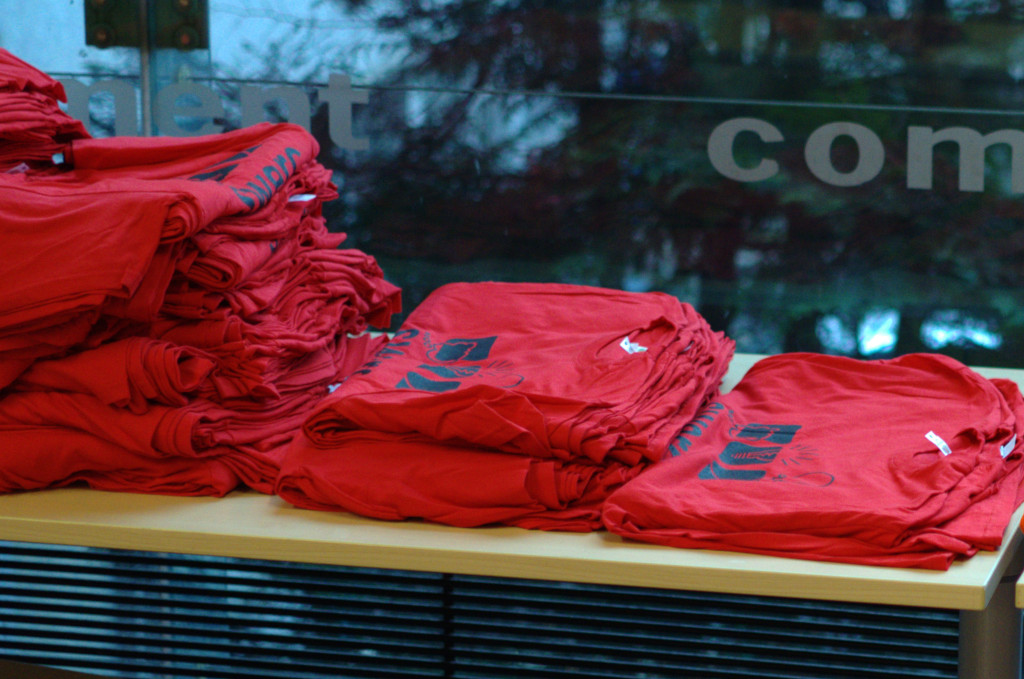
\includegraphics[width=\linewidth]{figs/tshirts}
    \end{minipage}
    
    \textbf{Entrée}\quad
    \textit{Ligne 1:} nombre de t-shirts de chaque taille.
    \textit{Ligne 2:} $n$, le nombre de participants.
    \textit{$n$ lignes suivantes:} choix de chaque participant.
    
    \textbf{Limites}\quad
    $n \leq 10^5$ et nombre total de t-shirts $\leq 10^5$.
    Temps : 1\,s.
    
    \textbf{Sortie}\quad
    \enquote{NO} s’il n’y a pas de solution, sinon \enquote{YES} suivi d’une des solutions possibles.
    
    \vspace{1em}
    \scriptsize\emph{Tiré de Technocup 2017 — Elimination Round 1}
\end{frame}
}

\begin{frame}{Modélisation comme un flot}
    \begin{minipage}{\dimexpr.3\textwidth-1em}
        \ttfamily
        0 1 0 1 1 0\\
        3\\
        XL\\
        S,M\\
        XL,XXL
    \end{minipage}\hfill\pause%
    \begin{minipage}{\dimexpr.7\textwidth-1em}
        \raggedleft
        \begin{tikzpicture}[>=Latex]
            \node[graph node] (s) at (0, 0) {$s$};
            \node[graph node, minimum width=2.8em, minimum height=2.8em]
                (S) at (-2.25, -1.5) {S};
            \node[graph node, minimum width=2.8em, minimum height=2.8em]
                (M) at (-0.75, -1.5) {M};
            \node[graph node, minimum width=2.8em, minimum height=2.8em]
                (XL) at (0.75, -1.5) {XL};
            \node[graph node, minimum width=2.8em, minimum height=2.8em]
                (XXL) at (2.25, -1.5) {XXL};
            
            \node[graph node] (P1) at (-1.5, -3) {P1};
            \node[graph node] (P2) at (0, -3) {P2};
            \node[graph node] (P3) at (1.5, -3) {P3};
            
            \node[graph node] (t) at (0, -4.5) {$t$};
            
            \draw[->] (s) -| node[pos=.75, weight, xshift=-8pt] {0} (S);
            \draw[->] (s) -| node[pos=.75, weight, xshift=-8pt] {1} (M);
            \draw[->] (s) -| node[pos=.75, weight, xshift=-8pt] {1} (XL);
            \draw[->] (s) -| node[pos=.75, weight, xshift=-8pt] {1} (XXL);
            
            \draw[->] (S.south) -- node[pos=.5, weight, xshift=-8pt] {1} (P2.north);
            \draw[->] (M.south) -- node[pos=.5, weight, xshift=-8pt] {1} (P2.north);
            \draw[->] (XL.south) -- node[pos=.5, weight, xshift=8pt] {1} (P1.north);
            \draw[->] (XL.south) -- node[pos=.5, weight, xshift=-8pt] {1} (P3.north);
            \draw[->] (XXL.south) -- node[pos=.5, weight, xshift=-8pt] {1} (P3.north);
            
            \draw[->] (P1) |- node[pos=.25, weight, xshift=-8pt] {1} (t);
            \draw[->] (P2) -- node[pos=.5, weight, xshift=-8pt] {1} (t);
            \draw[->] (P3) |- node[pos=.25, weight, xshift=-8pt] {1} (t);
        \end{tikzpicture}
    \end{minipage}
\end{frame}

\section{Quelques problèmes associés}
\maketoc

\begin{frame}{Coupe minimale}
    \begin{itemize}
        \item \textbf{Coupe minimale :} Enlever des arêtes du graphe de sorte à déconnecter $s$ de $t$, en minimisant le poids des arêtes retirées.
    \end{itemize}
    
    {\centering
    \vspace{1em}
    \begin{tikzpicture}[x=2cm, >=Latex]
        \node[graph node] (s) at (0, 0) {$s$};
        \node[graph node] (1) at (1, 1) {$1$};
        \node[graph node] (2) at (2, 1) {$2$};
        \node[graph node] (3) at (1, -1) {$3$};
        \node[graph node] (4) at (2, -1) {$4$};
        \node[graph node] (t) at (3, 0) {$t$};
        
        \draw[
            ->,
        ] (s) -- node[
            midway, weight,
            yshift=12pt,
        ] {5/5} (1);
        
        \draw[
            ->,
        ] (s) -- node[
            midway, weight,
            yshift=-12pt,
        ] {2/4} (3);
        
        \draw[
            ->,
        ] (3) -- node[
            midway, weight,
            xshift=-12pt,
        ] {1/3} (1);
        
        \draw[
            ->,
            onslide=<2>{highlight},
        ] (1) -- node[
            midway, weight,
            yshift=12pt,
        ] {6/6} (2);
        
        \draw[
            ->,
            onslide=<2>{highlight},
        ] (3) -- node[
            midway, weight,
            yshift=-12pt,
        ] {1/1} (4);
        
        \draw[
            ->,
        ] (2) -- node[
            midway, weight,
            xshift=-12pt,
        ] {1/8} (4);
        
        \draw[
            ->,
        ] (2) -- node[
            midway, weight,
            yshift=12pt,
        ] {5/5} (t);
        
        \draw[
            ->,
        ] (4) -- node[
            midway, weight,
            yshift=-12pt,
        ] {2/2} (t);
    \end{tikzpicture}
    
    }
    
    \pause
    \begin{itemize}
        \item \textbf{Flot maximum = Coupe minimum}
        \item Le réseau ne peut pas supporter un flot plus important que celui d’une quelconque coupe. Une coupe ne peut pas être d’un poids inférieur à celui d’un quelconque flot.
    \end{itemize}
\end{frame}

\begin{frame}{Couplage maximal dans un biparti}
    \begin{itemize}
        \item \textbf{Biparti :} Composé de deux ensembles de sommets indépendants.
        \item \textbf{Couplage :} Ensemble d’arêtes non-adjacentes (\enquote{disjointes}).
    \end{itemize}
    
    {\centering
    \begin{tikzpicture}[>=Latex]
        \node[graph node] (1) at (0, 0) {1};
        \node[graph node] (2) at (0, -1) {2};
        \node[graph node] (3) at (0, -2) {3};
        \node[graph node] (4) at (0, -3) {4};
        \node[graph node] (5) at (3, 0) {5};
        \node[graph node] (6) at (3, -1) {6};
        \node[graph node] (7) at (3, -2) {7};
        \node[graph node] (8) at (3, -3) {8};
        
        \draw[onslide=<2-3>{->}, onslide=<3-4>{highlight}] (1) -- (5);
        \draw[onslide=<2-3>{->}, onslide=<3-4>{highlight}] (2) -- (7);
        \draw[onslide=<2-3>{->}] (3) -- (5);
        \draw[onslide=<2-3>{->}] (3) -- (6);
        \draw[onslide=<2-3>{->}, onslide=<3-4>{highlight}] (3) -- (8);
        \draw[onslide=<2-3>{->}] (4) -- (7);
        
        \only<2-3>{
            \node[graph node] (s) at (-2, -1.5) {$s$};
            \node[graph node] (t) at (5, -1.5) {$t$};
            \draw[->, onslide=<3>{highlight}] (s) -- (1);
            \draw[->, onslide=<3>{highlight}] (s) -- (2);
            \draw[->, onslide=<3>{highlight}] (s) -- (3);
            \draw[->] (s) -- (4);
            \draw[->, onslide=<3>{highlight}] (5) -- (t);
            \draw[->] (6) -- (t);
            \draw[->, onslide=<3>{highlight}] (7) -- (t);
            \draw[->, onslide=<3>{highlight}] (8) -- (t);
        }
    \end{tikzpicture}
    
    }
\end{frame}

\begin{frame}{Exercices et références}
    \begin{itemize}
        \item Exercices:
        \begin{itemize}
            \item \href{https://codeforces.com/problemset/problem/727/D}{\textbf{Technocup 2017, “T-shirts Distribution”}}
            \item \href{https://onlinejudge.org/index.php?option=onlinejudge&page=show_problem&problem=1421}{UVa 10480, “Sabotage”}
        \end{itemize}
        \item Dans les livres de référence:
        \begin{itemize}
            \item Dürr et Vie, §9.5 à §9.8.
            \item Laaksonen, §12.3.
            \item Halim, §4.6.
        \end{itemize}
    \end{itemize}
\end{frame}

\end{document}